\documentclass{article}
\usepackage{graphicx}
\usepackage{hyperref}
\usepackage[czech]{babel}
\usepackage{csquotes}
\usepackage{tabularx}
\usepackage{changepage}

\title{IMP - Řízení spotřeby energie mikrokontroléru}
\author{Martin Slezák (xsleza26)}
\date{\today}

\begin{document}

\maketitle

\newpage

\tableofcontents

\newpage

\section{Úvod}

Tento projekt řeší řízení spotřeby energie mikrokontroléru, konkrétně na
mikrokontroléru FITkit3. Tento mikrokontrolér podporuje několik způsobů, jak
řídit spotřebu. V tomto projektu je popsáno, proč se spotřeba na
mikrokontroléru řídí a jak jednotlivé způsoby úspory energie fungují. Nakonec
na základě některých z těchto prostředků byla sestavena vestavěná aplikace.

\section{Proč řídit spotřebu}

Téměř v každé domácnosti se vyskytuje desítky mikrokontrolérů, které se mohou
vyskytovat například v pračce, lednici ale i v dalších mnoha zařízeních.

Mikrokontrolér v mnoha případech pouze čeká a samotná činnost se vykoná až
například po stisku klávesy nebo jednou za čas. V takové chvíli je zbytečné,
aby mikrokontrolér běžel, jelikož stále využívá energie.

\subsection{Jádro mikrokontroléru}

Jádro mikrokontroléru je nejvíce náročné na energii. Je tedy plýtváním energie
nechat jádro běžet zbytečně a nebo naopak moc rychle. V případě, že jádro čeká
na nějakou událost, se jádro uspí. Jakmile daná událost nastane, je jádro
probuzeno například přerušením (asynchronní) a nebo po uplynutí daného času
(synchronní).

Je však třeba najít ideální rychlost jádra. Moc velká frekvence jádra způsobí
větší spotřebu jádra, avšak akce bude dokončena rychleji a jádro lze poté
uspat, zatímco menší frekvence způsobí menší spotřebu, ale akce bude trvat
déle.

\subsection{Paměť}

Existují různé druhy paměti. Tyto paměti poté mají i různou spotřebu energie a
různou rychlost čtení či zápisu. Na základě těchto faktorů je vhodné zvolit
paměť, která nám bude dostačovat pro řešení našeho problému a bude mít možná co
nejmenší spotřebu. Například paměť RAM má menší spotřebu než paměť Flash. Tyto
rozdíly jsou však téměř zanedbatelné.

\subsection{Periferie}

Některé periferie nemusí být v aplikaci použiti, je proto vhodné vypnout jejich
hodinový signál, čímž periferii vypneme. V opačném případě, že periferii lze
použít pro řešení problému aplikace, je vhodné tuto periferii použít. Jak již
bylo zmíněno, jádro je nejvíce náročné na energie a je tedy vhodné
minimalizovat práci jádra.

\section{Základní pojmy}

\subsection{Nested Vectored Interrupt Controller (NVIC)}

NVIC je klíčová komponenta ARM procesorů, která řídí zpracovávání přerušení
v procesoru.

\subsection{Low-Leakage Wakeup Unit (LLWU)}

LLWU je periferní modul na čipu, který umožňuje interní periferie a externí
vstupní piny jako zdroj probuzení z režimů Low-Leakage (LLS a VLLSx).

\subsection{System Mode Controller (SMC)}

SMC (řadič systémového režimu) je zodpovědný za řazení systému do a ze všech
režimů Stop a Run s nízkou spotřebou. Monitoruje události pro spouštění
přechodů mezi režimy napájení a zároveň ovládá napájení, hodiny a paměti
systému, aby se dosáhlo spotřeby energie a funkčnosti daného režimu.

\subsection{General Purpose Input/Output (GPIO)}

GPIO referuje na piny na mikrokontroléru, které mohou být konfigurovány jako
vstup nebo výstup pro různé digitální signály.

\subsection{Analog-to-Digital Converter (ADC)}

ADC je periferní zařízení v mikrokontrolérech, které převádí analogový signál
na digitální hodnotu, kterou lze zpracovat pomocí mikrokontroléru.

\subsection{Real-Time Clock (RTC)}

RTC je periferie pro měření času v mikrokontrolérech, která uchovává aktální
datum a čas, i když je mikrokontrolér vypnutý. Využívá pro to vyhrazený zdroj
hodinového signálu s nízkou spotřebou.

\subsection{SRAM\_U a SRAM\_L}

Jedná se o různé sekce statické RAM v mikrokontroléru, typicky rozlišné na
základě jejich lokace nebo použití.
\begin{itemize}
    \item \textbf{SRAM\_U} (Upper SRAM) = horní část SRAM, typicky užívaná pro
        univerzální ukládání dat, proměnných a zásobníkových operací
    \item \textbf{SRAM\_L} (Lower SRAM) = spodní část SRAM, využíváná pro
        speciální účely, jako jsou spouštěcí data, konfigurace nebo specifické
        systémové proměnné
\end{itemize}

\section{Řízení spotřeby}

Mikrokontrolér obsahuje řadič správy napájení, který nabízí různé možnosti, jak
řídit spotřebu energie. Tato úspora je na základě požadované úrovně funkčnosti,
například zda je třeba zachovávat stav mikrokontroléru, případně vypnutí
logických obvodů. Stavy I/O (vstupy a výstupy) jsou však zachovány ve všech
režimech.

Na základě těchto nároků je zvolen jeden z existujících režimů. Tyto režimy
jsou děleny na základě ůrovně spotřeby, kdy agresivnější režimy omezí více
funkcionality.

Existují tři hlavní režimy činnosti: běhový (run), čekací (wait), zastavovací
(stop). Pomocí instrukce WFI (Wait For Interrupt) se čip přepne do čekacího
nebo zastavovacího režimu.

Pro každý běhový (run) režim existují odpovídající čekací (wait) a zastavovací
(stop) režimy. Čekací (wait) režim se podobá režimu spánku procesorů ARM.
Zastavovací (stop) jsou podobné hlubokému spánku ARM procesorů.

Existuje také režim velmi nízkého výkonu (VLPR), který umožňuje výrazně snížit
spotřebu během provozu v případě, že aplikace nepotřebuje maximální frekvenci
sběrnice.

\subsection{Normální režim}

\begin{tabularx}{\textwidth}{|>{\centering\arraybackslash}p{0.09\textwidth}|X|}
    \hline
    \textbf{Režim} & \textbf{Popis} \\
    \hline
    Run & Maximální výkon čipu. Defaultní režim po resetu. Zapnutý regulátor
    napětí \\
    \hline
    Wait & Jádro je uspané, periferie fungují. NVIC zůstává citlivý na
    přerušení \\
    \hline
    Stop & Čip v statickém stavu. Režim nejnižší spotřeby zachovávající stavy
    všech registrů. NVIC je zakázán, AWIC k probuzení z přerušení. Periferie
    nefungují \\
    \hline
\end{tabularx}

\subsection{Režim velmi nízkého výkonu}

\begin{tabularx}{\textwidth}{|>{\centering\arraybackslash}p{0.09\textwidth}|X|}
    \hline
    \textbf{Režim} & \textbf{Popis} \\
    \hline
    Run & Regulátor napětí v režimu nízké spotřeby (dostatek energie pro
    provoz při snížené frekvenci). Snížená frekvence režimu přístupu Flash.
    LVD vypnuto. Interní oscilátor poskytuje nízkovýkonový 4 MHz zdroj pro
    jádro, sběrnici a také periferie \\
    \hline
    Wait & Stejné jako run s jádrem v režimu spánku \\
    \hline
    Stop & Čip v statickém stavu, vypnutý provoz LVD. Režim nejnižší spotřeby
    ADC a funkčním přerušením pinů. Periferie nefungují, lze využít RTC,
    CMP,... NVIC je zakázán, AWIC k probuzení z přerušení. \\
    \hline
\end{tabularx}

\subsection{Low Leakage a Very Low Leakage}

\begin{tabularx}{\textwidth}{|>{\centering\arraybackslash}p{0.13\textwidth}|X|}
    \hline
    \textbf{Režim} & \textbf{Popis} \\
    \hline
    Low Leakage Stop & Stav zachování režimu napájení. Většina periferií v
    režimu zachování stavu (zastavené hodiny). NVIC zakázáno. LLWU k probuzení.
    \\
    \hline
    Very Low Leakage Stop3 & Většina periferií deaktivována. NVIC zakázáno.
    LLWU k probuzení. SRAM\_U a SRAM\_L zapnuté (obsah zachován) \\
    \hline
    Very Low Leakage Stop2 & Většina periferií deaktivována. NVIC zakázáno.
    LLWU k probuzení. SRAM\_L vypnutý. Část SRAM\_U zapnutá (obsah zachován).\\
    \hline
    Very Low Leakage Stop1 & Většina periferií deaktivována. NVIC zakázáno.
    LLWU k probuzení. Všechny SRAM\_U a SRAM\_L jsou vypnuté 32B soubor
    systémového registru a 32B soubor registru VBAT napájeny (data kritická
    pro zákazníky) \\
    \hline
\end{tabularx}

\newpage

\section{Přechody mezi režimy}

Přechody mezi režimy hezky znázorňuje následující stavový diagram. Z diagramu
lze vidět, že po resetu je mikrokontrolér v režimu Run, ze kterého poté může
přecházet do jednotlivých režimů. Navíc jsou ještě přechody mezi stavem Very
Low Power Run a jeho odpovídajícími Wait a Stop režimy. Z režimu VLPR lze také
přejít do režimů Very Low Leakage StopN (VLLS3, VLLS2, VLLS1) a Low Leakage
Stop (LLS).

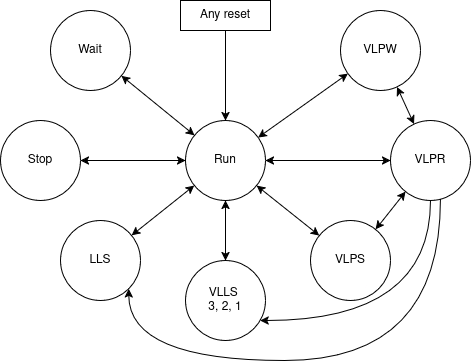
\includegraphics[width=1.0\textwidth]{power-modes.png}

Pro přechod do režimů Wait a Stop se využívá instrukce \texttt{WFI}, která se z
C programu volá pomocí funkce \texttt{\_\_WFI()}. Na základě nastavených hodnot
se přepne do odpovídajícího režimu.

\newpage
\section{Provoz modulů v režimech nízké spotřeby}

Následující tabulka ukazuje funkcionalitu jednotlivých modulů, zatímoc je čip
v režimu nízko spotřeby.

Návrat do režimu Run je proveden automaticky po přijmutí přerušení, přerušení
probuzení nebo reset probuzení. Čím hlubší režim spánku, tím je sice menší
spotřeba, ale zároveň i trvá déle mikrokontrolér probudit. Například jestliže
se vypne generátor hodin, trvá nějakou dobu, než bude produkovat stabilní
hodinový signál. Z nejhlubšího spánku se mikrokontrolér může probouzet velmi
dlouho, třeba i stovky \(\mu s\).

\subsection*{Použité názvy}
\begin{itemize}
    \item \textbf{FF} = Full Functionality (plná funkčnost)
    \item \textbf{static} = stavy registrů a pamětí jsou zachovány
    \item \textbf{powered} = paměť je napájena pro zachování obsahu
    \item \textbf{LP} = Low Power - Flash má stav nízké spotřeby uchovávající
        konfigurační registry pro podporu rychlejšího probuzení
    \item \textbf{OFF} = modul není napájen, po probuzení je ve stavu Reset
    \item \textbf{wakeup} = modul může sloužit jako zdroj probuzení čipu
\end{itemize}

\begin{table}[h]
\begin{adjustwidth}{-2.8cm}{1cm}
\begin{tabular}{ | c | c | c | c | c | c | c | }
    \hline
    \textbf{Modul} & \textbf{Stop} & \textbf{VLPR} & \textbf{VLPW} &
    \textbf{VLPS} & \textbf{LLS} & \textbf{VLLSx} \\
    \hline
    NVIC & static & FF & FF & static & static & OFF \\
    \hline
    Ovladač režimů & FF & FF & FF & FF & FF & FF \\
    \hline
    LLWU & static & static & static & static & FF & FF \\
    \hline
    Regulátor & ON & LP & LP & LP & LP & LP \\
    \hline
    Hodiny jádra & OFF & 4 MHz max & OFF & OFF & OFF & OFF \\
    \hline
    Systémové hodiny & OFF & 4 MHz max & 4 MHz max & OFF & OFF & OFF \\
    \hline
    Hodiny sběrnice & OFF & 4 MHz max & 4 MHz max & OFF & OFF & OFF \\
    \hline
    Flash & powered & 1 MHz max & LP & LP & OFF & OFF \\
    \hline
    Část SRAM\_U & LP & LP & LP & LP & LP & LP (VLLS3,2), OFF \\
    \hline
    RTC & FF & FF & FF & FF & FF & FF \\
    \hline
    ADC & Interní hodiny & FF & FF & Interní hodiny & static & OFF \\
    \hline
    GPIO & wakeup & FF & FF & wakeup & static & OFF \\
    \hline
\end{tabular}
\end{adjustwidth}
\caption{Tabulka provozu některých modulů v režimech nízké spotřeby}
\end{table}

\newpage
\section{Implementace}

Program implementuje přechody mezi některými režimy nízké spotřeby. Přepnutí
do režimu nízké spotřeby lze pomocí tlačítka. Tlačítka vyvolají přerušení,
ve kterém se poté nastaví hodnoty do specifických registrů. Konkrétní režim pro
konkrétní tlačítko je dán tímto seznamem:
\begin{itemize}
    \item SW2 - Very-Low-Leakage Stop1
    \item SW3 - Low-Leakage Stop
    \item SW4 - Low-Power Stop
    \item SW5 - Normal Stop
    \item SW6 - Normal Wait
\end{itemize}

V hlavním cyklu programu je kód pro blikání LED diody na desce mikrokontroléru.
Díky této LED lze poznat, zda jádro běží či nikoliv.

\newpage
\begin{thebibliography}{9}

\bibitem{reference-manual} Refereční manuál K60 Sub-Family, Kinetis.
\url{https://www.digikey.jp/htmldatasheets/production/1228931/0/0/1/K60-LQ-MD10-Ref-Manual.pdf}

\bibitem{imp-lectures} Přednášky předmětu IMP, VUT FIT

\end{thebibliography}

\end{document}
